
\chapter{Introduction}
\label{ch:introduction}
\todo[inline, backgroundcolor=kth-lightblue]{svensk: Introduktion}


\todo[inline, backgroundcolor=kth-lightblue]{Ofta kommer problemet och problemägaren
  från industrin där man önskar en specifik lösning på ett specifikt
  problem. Detta är ofta ”för smalt” definierat och ger ofta en ”för smal”
  lösning för att resultatet skall vara intressant ur ett mer allmänt
  ingenjörsperspektiv och med ”nya” erfarenheter som resultat. Fundera
  tillsammans med projektets intressenter (student, problemägare och akademi)
  hur man skulle kunna använda det aktuella problemet/förslaget för att
  undersöka någon ingenjörsaspekt och vars resultat kan ge ny eller
  kompletterande erfarenhet till ingenjörssamfundet och vetenskapen.\\
  
  Examensarbetet handlar då om att ta fram denna nya ”erfarenhet” och på köpet
  löser man en del eller hela delen av det ursprungliga problemet.\\

  Erfarenheten kommer ur en frågeställning som man i examensarbetet försöker
  besvara med tidigare och andras erfarenhet, egna eller modifierade metoder som
  ger ett resultat vilket kan användas för att diskutera ett svar på
  undersökningsfrågan.\\

  Detta stycke skall alltså, förutom det ursprungliga ”smala” problemet,
  innehålla  vad som skall undersökas för att skapa ny ingenjörserfarenhet
  och/eller vetenskap.
}

\todo[inline, backgroundcolor=kth-lightgreen]{The first paragraph after a heading is not indented, all of the
  subsequent paragraphs have their first line indented.}
  
This chapter describes the specific problem that this thesis addresses, the context of the problem, the
goals of this thesis project, and outlines the structure of the thesis.\\

\todo[inline]{Give a general introduction to the area. (Remember to use appropriate references in this and all other sections.)}

% One can use either biblatex or bibtex - set as the option for the document at the top of this file
\ifbiblatex
\todo[inline, backgroundcolor=kth-lightgreen]{We use the \emph{biblatex} package to handle our references.  We
use the command \texttt{parencite} to get a reference in parenthesis, like
this \textbackslash parencite\{heisenberg2015\} resulting in \parencite{heisenberg2015}.  It is also possible to include the author as part of the sentence using \texttt{textcite}, like talking about the work of \textbackslash textcite\{einstein2016\} resulting in \textcite{einstein2016}.\\
This also means that you have to change the include files to include biblatex and change the way that the reference.bib file is included.}
\else
\todo[inline, backgroundcolor=kth-lightgreen]{We use the \emph{bibtex} package to handle our references.  We therefore
use the command \textbackslash cite\{farshin\_make\_2019\}. For example, Farshin, \etal described how to improve LLC
cache performance in \cite{farshin_make_2019} in the context of links running
at \SI{200}{Gbps}.}
\fi

\todo[inline, backgroundcolor=kth-lightgreen]{Use the glossaries package to help yourself and your readers.
Add the acronyms and abbreviations to templates/kth/lib/acronyms.tex. Some examples are shown below:}
In this thesis we will examine the use of \glspl{LAN}. In this thesis we will
assume that \glspl{LAN} include \glspl{WLAN}, such as \gls{WiFi}.


\section{Background}
\label{sec:background}
\todo[inline, backgroundcolor=kth-lightblue]{svensk: Bakgrund}

\todo[inline]{Present the background for the area. Set the context for your project – so that your reader can understand both your project and this thesis. (Give detailed background information in Chapter 2 - together with related work.)
Sometimes it is useful to insert a system diagram here so that the reader
knows what are the different elements and their relationship to each
other. This also introduces the names/terms/… that you are going to use
throughout your thesis (be consistent). This figure will also help you later
delimit what you are going to do and what others have done or will do.}

As one can find in RFC 1235\,\cite{ioannidis_coherent_1991} multicast is useful for xxxx. A number of different \glspl{OS} have been used in this work, such as the following \glspl{OS}: UNIX, Linux, Windows, etc. The main focus will be on one \gls{OS}, namely Linux.

\section{Problem}
\label{sec:problem}
\todo[inline, backgroundcolor=kth-lightblue]{svensk: Problemdefinition eller Frågeställning\\
Lyft fram det ursprungliga problemet om det finns något och definiera därefter
den ingenjörsmässiga erfarenheten eller/och vetenskapen som kan komma ur
projektet. }

Longer problem statement\\
If possible, end this section with a question as a problem statement.

% Research Question
\subsection{Original problem and definition}
\label{sec:researchQuestion}
\todo[inline, backgroundcolor=kth-lightblue]{Ursprungligt problem och definition}
Some text

\subsection{Scientific and engineering issues}\todo[inline, backgroundcolor=kth-lightblue]{Vetenskaplig och ingenjörsmässig frågeställning}
some text

\section{Purpose}
\todo[inline, backgroundcolor=kth-lightblue]{Syfte}
\todo[inline, backgroundcolor=kth-lightblue]{Skilj på syfte och mål! Syfte är att förändra något till det bättre. I examensarbetet finns ofta två aspekter på detta. Dels vill problemägaren (företaget) få sitt problem löst till det bättre men akademin och ingenjörssamfundet vill också få nya erfarenheter och vetskap. Beskriv ett syfte som tillfredställer båda dessa aspekter.\\
Det finns även ett syfte till som kan vara värt att beakta och det är att du som student skall ta examen och att du måste bevisa, i ditt examensarbete, att du uppfyller examensmålen. Dessa mål sammanfaller med kursmålen för examensarbetskursen. 
}
\todo[inline]{State the purpose  of your thesis and the purpose of your degree project.\\
Describe who benefits and how they benefit if you achieve your goals. Include anticipated ethical, sustainability, social issues, etc. related to your project. (Return to these in your reflections in Section~\ref{sec:reflections}.)}



\section{Goals}
\todo[inline, backgroundcolor=kth-lightblue]{Mål}
\todo[inline, backgroundcolor=kth-lightblue]{Skilj på syfte och mål. Syftet är att åstakomma en förändring i något. Målen är vad som konkret skall göras för att om möjligt uppnå den önskade förändringen (syfte). }

\todo[inline]{State the goal/goals of this degree project.}

The goal of this project is XXX. This has been divided into the following three sub-goals:
\begin{enumerate}
\item Subgoal 1 \todo[inline, backgroundcolor=kth-lightblue]{för att tillfredsställa problemägaren – industrin?}
\item Subgoal 2\todo[inline, backgroundcolor=kth-lightblue]{för att tillfredsställa ingenjörssamfundet och vetenskapen – akademin) }
\item Subgoal 3\todo[inline, backgroundcolor=kth-lightblue]{eventuellt, för att uppfylla kursmålen – du som student}
\end{enumerate}

\todo[inline]{In addition to presenting the goal(s), you might also state what the deliverables and results of the project are.}

\section{Research Methodology}\todo[inline, backgroundcolor=kth-lightblue]{Undersökningsmetod}
\todo[inline, backgroundcolor=kth-lightblue]{Här anger du vilken vilken övergripande undersökningsstrategi eller metod du skall använda för att försöka besvara den akademiska frågeställning och samtidigt lösa det e v ursprungliga problemet. Ofta kan man använda ”lösandet av ursprungsproblemet” som en fallstudie kring en akademisk frågeställning. Du undersöker någon intressant fråga i ”skarpt” läge och samlar resultat och erfarenhet ur detta.\\
Tänk på att företaget ibland måste stå tillbaka i sin önskan och förväntan på projektets resultat till förmån för ny eller kompletterande ingenjörserfarenhet och vetenskap (ditt examensarbete). Det är du som student som bestämmer och löser fördelningen mellan dessa två intressen men se till att alla är informerade. }
\todo[inline]{Introduce your choice of methodology/methodologies and method/methods – and the reason why you chose them. Contrast them with and explain why you did not choose other methodologies or methods. (The details of the actual methodology and method you have chosen will be given in Chapter~\ref{ch:methods}. Note that in Chapter~\ref{ch:methods}, the focus could be research strategies, data collection, data analysis, and quality assurance.)\\
In this section you should present your philosophical assumption(s), research method(s), and research approach(es).}

\section{Delimitations}\todo[inline, backgroundcolor=kth-lightblue]{Avgränsningar}
\todo[inline]{Describe the boundary/limits of your thesis project and what you are explicitly not going to do. This will help you bound your efforts – as you have clearly defined what is out of the scope of this thesis project. Explain the delimitations. These are all the things that could affect the study if they were examined and included in the degree project.}

\section{Structure of the thesis}\todo[inline, backgroundcolor=kth-lightblue]{ Rapportens disposition}
Chapter~\ref{ch:background} presents relevant background information about xxx.  Chapter~\ref{ch:methods} presents the methodology and method used to solve the problem. …

\cleardoublepage
\chapter{Background}

\chapter{Background}

\label{ch:background}
% \todo[inline, backgroundcolor=kth-lightblue]{Bakgrund}

% \todo[inline]{When you do your literature study, you should have a nearly complete Chapters 1 and 2.\\
% You may also find it convenient to introduce the future work section into your report early – so that you can put things that you think about but decide not to do now into this section.\\
% Note that later you can move things between this future work section and what you have done as you may change your mind about what to do now versus what to put off to future work.
% }
% \todo[inline]{What does a reader (another x student -- where x is your study line) need to know to understand your report?
% What have others already done? (This is the “related work”.) Explain what and
% how prior work / prior research will be applied on or used in the degree
% project /work (described in this thesis). Explain why and what is not used in
% the degree project and give valid reasons for rejecting the work/research.}

This chapter provides basic background information about xxx. Additionally, this chapter describes xxx. The chapter also describes related work xxxx.



% \todo[inline, backgroundcolor=kth-lightblue]{Vilken viktig litteratur och
  % (forsknings-)artiklar har du studerat inom området (litteraturstudie)? }

\section{Filesystems}
Filesystems are used to store data on for instance a hard drive of a computer on in the cloud. Google Drive is a filesystem that enables user to save their data online up to 15 GB for free\cite{CloudStorageWork} using their clusters of distributed storage devices, meaning that the data is saved on theirs servers which can be located wherever\cite{DistributedStorageWhat}. Paying customers can achieve higher amount of storage using the service.

A deniable filesystem is a system that does not expose files stored on this system without credentials - neither how many files are stored, their sizes, their content or even if there exists any files on the filesystem\cite{petersDEFYDeniableFile2014}. This is useful if for example one is to be exposed to an audit of their data by a totalitarian regim where they don't even want to disclose that they have data.

A unix filesystem uses a data structure called an \textit{inode}. An inode keeps track of the metadata for the files in the filesystem, and a directory simply contains the file names, and each files/directory's inode id. Using a lookup, the system can then learn about the file - where it is located, for instance how big it is, as can be seen in Figure~\ref{fig:inode_diag} (\textbf{CITATION NEEDED}). Each inode entry can contain any number of metadata information which might be relevant for the system, such as creation time and last updated.

\begin{figure}[!ht]
	\begin{center}
	  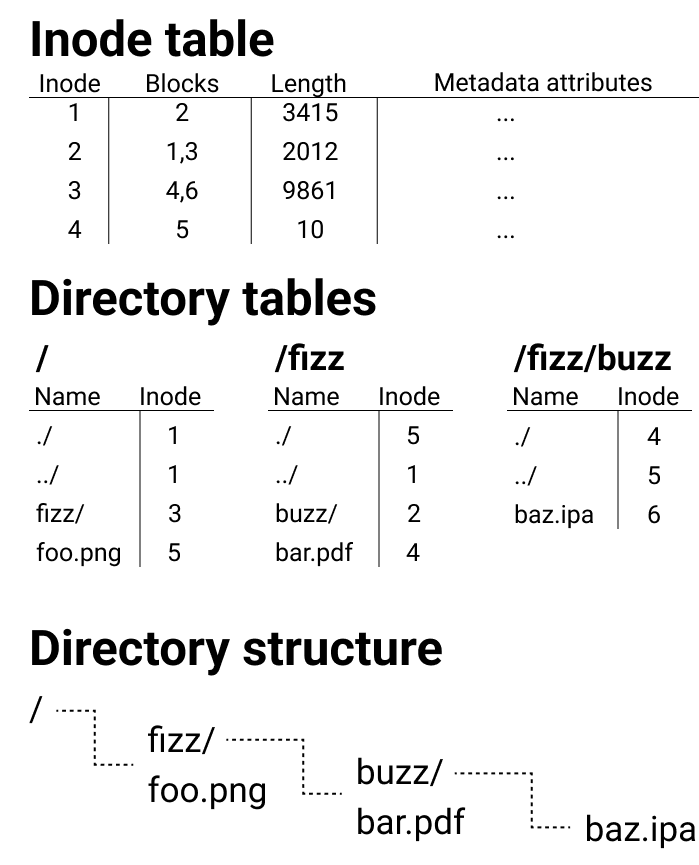
\includegraphics[width=0.8\textwidth]{figures/inode_diagram.png}
	\end{center}
	\caption{Basic structure of inode based filesystem}
	\label{fig:inode_diag}
\end{figure}

Looking at the 4 main file systems of windows, they all have many, sometimes different, functionalities such as links and named streams as well limitations such as a defined theoretical maximum file size\cite{mikbenFileSystemFunctionality}. This is set to 16 exbibytes for NTFS, exFAT and UDF, and for FAT32 it is set to 4 gigabytes. 

\section{Twitter}
\label{sec:twitter}
Twitter is a micro-blog online where users can sign up for a free account and create public posts (tweets) using text, images, and videos. Each post has a unique id associated with it\,\cite{twitterTwitterIDs}. Text posts are limited to $280$ characters while images can be up to \SI{5}{\mega\byte} and videos up to \SI{512}{\mega\byte}\,\cite{MediaBestPractices}. An post with images can contain up to 4 images in one post. There is also a possibility to send private messages to other accounts, where each message can contain up to $10\,000$ characters and the same limitations on files. However, direct messages older than $30$ days are not possible to retrieve through Twitter's API\,\cite{RetrievingOlder302018}. It is possible to create threads of Twitter posts where multiple tweets can be associated in chronological order.

Twitter's API defines technical limits of how many times certain actions can be executed by a user\,\cite{UnderstandingTwitterLimits}. A maximum of $2\,400$ tweets can be sent per day, and the limit is further broken down into smaller limits at semi-hourly intervals. Hitting a limit means that the user account no longer can perform the actions that the limit represents until the time period has elapsed.

\section{Related Work}
\citeauthor{peters_defy_2014} created a deniable filesystem using a log-based structure in \citeyear{peters_defy_2014}\cite{peters_defy_2014}. The filesystem of my project could be seen as a deniable system in the sense that the data is not actually stored on the device, and if the filesystem is not mounted it could be hard to prove that the user actually has data, even if they for instance would find the twitter account. This was also developed using FUSE\cite{noauthor_libfuse_2021} which I also will be using.

% \section{Major background area 1}
% \todo[inline, backgroundcolor=kth-lightblue]{Viktigt bakgrundsområde 1}
There are xxx characteristics that distinguish yyy from other information and communication technology (ICT) system, as shown in Figure~\ref{fig:lotsofstars}. Table \ref{tab:tablecaracteristics} summarizes these characteristics.

 
\begin{figure}[!ht]
  \begin{center}
    
\includegraphics[width=0.5\textwidth]{figures/lots_of_stars.png}
  \end{center}
  \caption{Lots of stars  (Inspired by Figure x.y on page z of [xxx])}
  \label{fig:lotsofstars}
\end{figure}
% \todo[inline, backgroundcolor=kth-lightblue]{Massor av stärnor (Inspirerad av figur x.y på sidan z i [xxx])}


\begin{table}[!ht]
  \begin{center}
    \caption{xxx characteristics}
    \label{tab:tablecaracteristics}
    \begin{tabular}{l|S[table-format=4.6]} % <-- Alignments: 1st column left, 2nd middle, with vertical lines in between
      \textbf{Characteristics} & \textbf{Description}\\
      $\alpha$ & $\beta$ \\
      \hline
      1 & 1110.1\\
      2 & 10.1\\
      3 & 23.113231\\
    \end{tabular}
  \end{center}
\end{table}
% \todo[inline, backgroundcolor=kth-lightblue]{Egenskaper}
% \todo[inline, backgroundcolor=kth-lightblue]{ Beskrivning}

\subsection{Subarea 1.1}
Entangled states are an important part of quantum cryptography, but also relevant in other domains. This concept might be relevant for neutrinos, see for example \cite{kim_small-mass_2016}.

\subsection{Subarea 1.1.2}
Computational methods are increasingly used as a third method of carrying out
scientific investigations. For example, computational experiments were used to
find the amount of wear in a polyethylene liner of a hip prosthesis in \cite{maguire_jr_new_2014}.
…

\subsection{Subarea 1.1.2}
Using the nearest data center may improve performance, see \cite{bogdanov_nearest_2015}


\subsection{Link layer Encapsulation}
\label{sec:llencap}

% See Figure~\ref{fig:ieee8023-data-packet} which uses the \textsf{bytefield}  \LaTeX\ package. 


% \begin{figure}[!ht]
% 	\centering
% \begin{bytefield}{21}
% \bitbox[]{7}{} & \bitbox[]{3}{\tiny octets:} & \bitbox[]{4}{\tiny 6} & \bitbox[]{4}{\tiny 6} & \bitbox[]{3}{\tiny 2} & \bitbox[]{5}{\tiny 46 to 1500} & \bitbox[]{3}{\tiny 0 to 46} & \bitbox[]{2}{\tiny 4}\\ 

% \bitbox[]{8}{\textbf{ETHERNET \\[-1ex] \tiny{data link-layer}}} & \bitbox[]{2}{} & 

% \bitbox{4}{\tiny Destination Address} & \bitbox{4}{\tiny Source Address} & \bitbox{3}{\tiny Length/ Type} & 
% \bitbox{5}{\tiny Data Payload} & \bitbox{3}{\tiny Padding} &
% \bitbox{2}{\tiny CRC} \\

% \bitbox[]{1}{} &\bitbox[]{3}{\tiny octets:} & \bitbox[]{4}{\tiny 7} & \bitbox[]{2}{\tiny 1} & \bitbox[]{0}{$\vdots$ \\[1ex]} & \bitbox[]{16}{} & \bitbox[]{0}{$\vdots$ \\[1ex]} & \bitbox[]{5}{} & \bitbox[]{4}{\tiny Variable}\\

% \bitbox[]{4}{\textbf{MAC \\[-1ex] \tiny{packet}}} & \colorbitbox{lightgray}{4}{\tiny Preamble} & \colorbitbox{lightgray}{2}{\tiny SFD} & \colorbitbox{lightgray}{16}{\tiny MAC Client Data} & \colorbitbox{lightgray}{3}{\tiny Padding} &
% \colorbitbox{lightgray}{2}{\tiny CRC} & \colorbitbox{lightgray}{4}{\tiny Extension}
% \end{bytefield}
%      \label{fig:ieee8023-data-packet}
%      \caption{Ethernet data link layer protocol encapsulated into a IEEE~802.3 MAC packet}
% \end{figure}

\subsection{IP packet headers}
\label{sec:ipheaders}
% The data link layer will receive a packet from the IP layer. The layout of
% an IPv4 packet is shown in Figure~\ref{fig:ipv4-header}. This should be
% contrasted with the IPv6 header shown in Figure~\ref{fig:ipv6-header}.

%
% IPv4 packet header
%
% \begin{figure}[!ht]
% 	\centering
% \begin{bytefield}{32}
% \bitheader{0-31} \\
% \bitbox{4}{\footnotesize{Version}} & \bitbox{4}{IHL} & \bitbox{6}{\tiny{Type of Service}} & \bitbox{2}{{\scriptsize ECN}} \bitbox{16}{Total Length}\\
% \bitbox{16}{Identification} & \bitbox{3}{Flags} & \bitbox{13}{Fragment Offset}\\
% \bitbox{8}{Time to Live} & \bitbox{8}{Protocol} & \bitbox{16}{Header Checksum}\\
% \wordbox{1}{Source Address}\\
% \wordbox{1}{Destination Address}\\
% \colorbitbox{lightgray}{24}{Options} & \colorbitbox{lightgray}{8}{Padding}
% \end{bytefield}
%      \label{fig:ipv4-header} 
%      \caption[IPv4 datagram header]{IPv4 datagram header. Light grey coloured fields are optional.}
% \end{figure}

%
% IPv6 packet header
%
% \begin{figure}[!ht]
% 	\centering
% \begin{bytefield}{32}
% \bitheader{0-31} \\
% \bitbox{4}{\footnotesize{Version}} & \bitbox{8}{Traffic Class} & \bitbox{20}{Flow Label}\\
% \bitbox{16}{Payload Length} & \bitbox{8}{Next Header} & \bitbox{8}{Hop Limit}\\
% \wordbox{4}{Source Address}\\
% \wordbox{4}{Destination Address}\\
% \end{bytefield}
%      \label{fig:ipv6-header}
%      \caption{IPv6 datagram header}
% \end{figure}

\subsection{Test for accessibility of formulas}

As can be seen in these equations:
$c=2 \cdot \pi \cdot r$ or \[ \int_{a}^{b} x^2 \,dx \] a chemical formula: $(C_5O_2H_8)_n$
...

% 
\section{Major background area 2} % \todo[inline, backgroundcolor=kth-lightblue]{Viktigt bakgrundsområde 2}
...
\subsection{\glsentryshort{WLAN} Security}% you can't use the \gls macro in a heading - but you can get the short (\glsentryshort) or long version (\glsentryshort) or \glsentrylong or even the text entry (\glsentrytext) and then there is no problem - see https://tex.stackexchange.com/questions/198140/glossaries-and-custom-section-headings-broken

\section{Related work area} % \todo[inline, backgroundcolor=kth-lightblue]{Relaterade arbeten}


\subsection{Major related work 1} % \todo[inline, backgroundcolor=kth-lightblue]{Relaterade arbeten 1}
Carrier clouds have been suggested as a way to reduce the delay between the users and the cloud server that is providing them with content. However, there is a question of how to find the available resources in such a carrier cloud. One approach has been to disseminate resource information using an extension to OSPF-TE, see Roozbeh, Sefidcon, and Maguire \cite{roozbeh_resource_2013}.


\subsection{Major related work} % \todo[inline, backgroundcolor=kth-lightblue]{Relaterade arbeten}

\subsection{Minor related work 1} % \todo[inline, backgroundcolor=kth-lightblue]{Mindre relaterat arbete 1}


…
\subsection{Minor related work n} % \todo[inline, backgroundcolor=kth-lightblue]{Mindre relaterat arbete n}



% 
\section{Summary} % \todo[inline, backgroundcolor=kth-lightblue]{Sammanfattning}
% \todo[inline, backgroundcolor=kth-lightblue]{Det är trevligt om detta kapitel
%   avslutas med en sammanfattning. Till exempel kan du inkludera en tabell som
%   sammanfattar andras idéer och fördelar och nackdelar med varje - så som
%   senare kan du jämföra din lösning till var och en av dessa. Detta kommer
%   också att hjälpa dig att definiera de variabler som du kommer att använda
%   för din utvärdering.}

% \todo[inline]{It is nice to have this chapter conclude with a summary. For
%   example, you can include a table that summarizes other people's ideas and
%   benefits and drawbacks with each - so as later you can compare your solution
%   to each of them. This will also help you define the variables that you will
%   use for your evaluation.}

\label{ch:background}
\todo[inline, backgroundcolor=kth-lightblue]{Bakgrund}

\todo[inline]{When you do your literature study, you should have a nearly complete Chapters 1 and 2.\\
You may also find it convenient to introduce the future work section into your report early – so that you can put things that you think about but decide not to do now into this section.\\
Note that later you can move things between this future work section and what you have done as you may change your mind about what to do now versus what to put off to future work.
}
\todo[inline]{What does a reader (another x student -- where x is your study line) need to know to understand your report?
What have others already done? (This is the “related work”.) Explain what and
how prior work / prior research will be applied on or used in the degree
project /work (described in this thesis). Explain why and what is not used in
the degree project and give valid reasons for rejecting the work/research.}

This chapter provides basic background information about xxx. Additionally, this chapter describes xxx. The chapter also describes related work xxxx.



\todo[inline, backgroundcolor=kth-lightblue]{Vilken viktig litteratur och
  (forsknings-)artiklar har du studerat inom området (litteraturstudie)? }

\section{Major background area 1}
\todo[inline, backgroundcolor=kth-lightblue]{Viktigt bakgrundsområde 1}
There are xxx characteristics that distinguish yyy from other information and communication technology (ICT) system, as shown in Figure~\ref{fig:lotsofstars}. Table \ref{tab:tablecaracteristics} summarizes these characteristics.

 
\begin{figure}[!ht]
  \begin{center}
    
\includegraphics[width=0.5\textwidth]{figures/lots_of_stars.png}
  \end{center}
  \caption{Lots of stars  (Inspired by Figure x.y on page z of [xxx])}
  \label{fig:lotsofstars}
\end{figure}
\todo[inline, backgroundcolor=kth-lightblue]{Massor av stärnor (Inspirerad av figur x.y på sidan z i [xxx])}


\begin{table}[!ht]
  \begin{center}
    \caption{xxx characteristics}
    \label{tab:tablecaracteristics}
    \begin{tabular}{l|S[table-format=4.6]} % <-- Alignments: 1st column left, 2nd middle, with vertical lines in between
      \textbf{Characteristics} & \textbf{Description}\\
      $\alpha$ & $\beta$ \\
      \hline
      1 & 1110.1\\
      2 & 10.1\\
      3 & 23.113231\\
    \end{tabular}
  \end{center}
\end{table}
\todo[inline, backgroundcolor=kth-lightblue]{Egenskaper}
\todo[inline, backgroundcolor=kth-lightblue]{ Beskrivning}

\subsection{Subarea 1.1}
Entangled states are an important part of quantum cryptography, but also relevant in other domains. This concept might be relevant for neutrinos, see for example \cite{kim_small-mass_2016}.

\subsection{Subarea 1.1.2}
Computational methods are increasingly used as a third method of carrying out
scientific investigations. For example, computational experiments were used to
find the amount of wear in a polyethylene liner of a hip prosthesis in \cite{maguire_jr_new_2014}.
…

\subsection{Subarea 1.1.2}
Using the nearest data center may improve performance, see \cite{bogdanov_nearest_2015}


\subsection{Link layer Encapsulation}
\label{sec:llencap}

See Figure~\ref{fig:ieee8023-data-packet} which uses the \textsf{bytefield}  \LaTeX\ package. 


\begin{figure}[!ht]
	\centering
\begin{bytefield}{21}
\bitbox[]{7}{} & \bitbox[]{3}{\tiny octets:} & \bitbox[]{4}{\tiny 6} & \bitbox[]{4}{\tiny 6} & \bitbox[]{3}{\tiny 2} & \bitbox[]{5}{\tiny 46 to 1500} & \bitbox[]{3}{\tiny 0 to 46} & \bitbox[]{2}{\tiny 4}\\ 

\bitbox[]{8}{\textbf{ETHERNET \\[-1ex] \tiny{data link-layer}}} & \bitbox[]{2}{} & 

\bitbox{4}{\tiny Destination Address} & \bitbox{4}{\tiny Source Address} & \bitbox{3}{\tiny Length/ Type} & 
\bitbox{5}{\tiny Data Payload} & \bitbox{3}{\tiny Padding} &
\bitbox{2}{\tiny CRC} \\

\bitbox[]{1}{} &\bitbox[]{3}{\tiny octets:} & \bitbox[]{4}{\tiny 7} & \bitbox[]{2}{\tiny 1} & \bitbox[]{0}{$\vdots$ \\[1ex]} & \bitbox[]{16}{} & \bitbox[]{0}{$\vdots$ \\[1ex]} & \bitbox[]{5}{} & \bitbox[]{4}{\tiny Variable}\\

\bitbox[]{4}{\textbf{MAC \\[-1ex] \tiny{packet}}} & \colorbitbox{lightgray}{4}{\tiny Preamble} & \colorbitbox{lightgray}{2}{\tiny SFD} & \colorbitbox{lightgray}{16}{\tiny MAC Client Data} & \colorbitbox{lightgray}{3}{\tiny Padding} &
\colorbitbox{lightgray}{2}{\tiny CRC} & \colorbitbox{lightgray}{4}{\tiny Extension}
\end{bytefield}
     \label{fig:ieee8023-data-packet}
     \caption{Ethernet data link layer protocol encapsulated into a IEEE~802.3 MAC packet}
\end{figure}

\subsection{IP packet headers}
\label{sec:ipheaders}
The data link layer will receive a packet from the IP layer. The layout of
an IPv4 packet is shown in Figure~\ref{fig:ipv4-header}. This should be
contrasted with the IPv6 header shown in Figure~\ref{fig:ipv6-header}.

%
% IPv4 packet header
%
\begin{figure}[!ht]
	\centering
\begin{bytefield}{32}
\bitheader{0-31} \\
\bitbox{4}{\footnotesize{Version}} & \bitbox{4}{IHL} & \bitbox{6}{\tiny{Type of Service}} & \bitbox{2}{{\scriptsize ECN}} \bitbox{16}{Total Length}\\
\bitbox{16}{Identification} & \bitbox{3}{Flags} & \bitbox{13}{Fragment Offset}\\
\bitbox{8}{Time to Live} & \bitbox{8}{Protocol} & \bitbox{16}{Header Checksum}\\
\wordbox{1}{Source Address}\\
\wordbox{1}{Destination Address}\\
\colorbitbox{lightgray}{24}{Options} & \colorbitbox{lightgray}{8}{Padding}
\end{bytefield}
     \label{fig:ipv4-header} 
     \caption[IPv4 datagram header]{IPv4 datagram header. Light grey coloured fields are optional.}
\end{figure}

%
% IPv6 packet header
%
\begin{figure}[!ht]
	\centering
\begin{bytefield}{32}
\bitheader{0-31} \\
\bitbox{4}{\footnotesize{Version}} & \bitbox{8}{Traffic Class} & \bitbox{20}{Flow Label}\\
\bitbox{16}{Payload Length} & \bitbox{8}{Next Header} & \bitbox{8}{Hop Limit}\\
\wordbox{4}{Source Address}\\
\wordbox{4}{Destination Address}\\
\end{bytefield}
     \label{fig:ipv6-header}
     \caption{IPv6 datagram header}
\end{figure}

\subsection{Test for accessibility of formulas}

As can be seen in these equations:
$c=2 \cdot \pi \cdot r$ or \[ \int_{a}^{b} x^2 \,dx \] a chemical formula: $(C_5O_2H_8)_n$
...
\section{Major background area 2}\todo[inline, backgroundcolor=kth-lightblue]{Viktigt bakgrundsområde 2}
...
\subsection{\glsentryshort{WLAN} Security}% you can't use the \gls macro in a heading - but you can get the short (\glsentryshort) or long version (\glsentryshort) or \glsentrylong or even the text entry (\glsentrytext) and then there is no problem - see https://tex.stackexchange.com/questions/198140/glossaries-and-custom-section-headings-broken

\section{Related work area}\todo[inline, backgroundcolor=kth-lightblue]{Relaterade arbeten}


\subsection{Major related work 1}\todo[inline, backgroundcolor=kth-lightblue]{Relaterade arbeten 1}
Carrier clouds have been suggested as a way to reduce the delay between the users and the cloud server that is providing them with content. However, there is a question of how to find the available resources in such a carrier cloud. One approach has been to disseminate resource information using an extension to OSPF-TE, see Roozbeh, Sefidcon, and Maguire \cite{roozbeh_resource_2013}.


\subsection{Major related work}\todo[inline, backgroundcolor=kth-lightblue]{Relaterade arbeten}

\subsection{Minor related work 1}\todo[inline, backgroundcolor=kth-lightblue]{Mindre relaterat arbete 1}


…
\subsection{Minor related work n}\todo[inline, backgroundcolor=kth-lightblue]{Mindre relaterat arbete n}


\section{Summary}\todo[inline, backgroundcolor=kth-lightblue]{Sammanfattning}
\todo[inline, backgroundcolor=kth-lightblue]{Det är trevligt om detta kapitel
  avslutas med en sammanfattning. Till exempel kan du inkludera en tabell som
  sammanfattar andras idéer och fördelar och nackdelar med varje - så som
  senare kan du jämföra din lösning till var och en av dessa. Detta kommer
  också att hjälpa dig att definiera de variabler som du kommer att använda
  för din utvärdering.}

\todo[inline]{It is nice to have this chapter conclude with a summary. For
  example, you can include a table that summarizes other people's ideas and
  benefits and drawbacks with each - so as later you can compare your solution
  to each of them. This will also help you define the variables that you will
  use for your evaluation.}

\cleardoublepage
\chapter{Method or Methods}
\label{ch:methods}
\todo[inline, backgroundcolor=kth-lightblue]{Metod eller Metodval}
\todo[inline]{This chapter is about Engineering-related
  content, Methodologies and Methods.  Use a self-explaining title.\\The
  contents and structure of this chapter will change with your choice of
  methodology and methods.}



\todo[inline]{Describe the engineering-related contents (preferably with models) and the research methodology and methods that are used in the degree project.\\
Give a theoretical description of the scientific or engineering methodology are you going to use and why have you chosen this method. What other methods did you consider and why did you reject them.\\
In this chapter, you describe what engineering-related and scientific skills you are going to apply, such as modeling, analyzing, developing, and evaluating engineering-related and scientific content. The choice of these methods should be appropriate for the problem . Additionally, you should be consciousness of aspects relating to society and ethics (if applicable). The choices should also reflect your goals and what you (or someone else) should be able to do as a result of your solution - which could not be done well before you started.}

The purpose of this chapter is to provide an overview of the research method
used in this thesis. Section~\ref{sec:researchProcess} describes the research
process. Section~\ref{sec:researchParadigm} details the research
paradigm. Section~\ref{sec:dataCollection} focuses on the data collection
techniques used for this research. Section~\ref{sec:experimentalDesign}
describes the experimental design. Section~\ref{sec:assessingReliability}
explains the techniques used to evaluate the reliability and validity of the
data collected. Section~\ref{sec:plannedDataAnalysis} describes the method
used for the data analysis. Finally, Section~\ref{sec:evaluationFramework}
describes the framework selected to evaluate xxx.

\todo[inline, backgroundcolor=kth-lightblue]{Vilka vetenskaplig eller ingenjörs-metodik ska du använda och varför har du valt den här metoden. Vilka andra metoder gjorde du övervägde du och varför du avvisar dem.
Vad är dina mål? (Vad ska du kunna göra som ett resultat av din lösning - vilken inte kan göras i god tid innan du började)
Vad du ska göra? Hur? Varför? Till exempel, om du har implementerat en artefakt vad gjorde du och varför? Hur kommer du utvärdera den.
Syftet med detta kapitel är att ge en översikt över forsknings metod som
används i denna avhandling. Avsnitt~\ref{sec:researchProcess} beskriver forskningsprocessen. Avsnitt~\ref{sec:researchParadigm} beskriver forskningsparadigmen detaljerat. Avsnitt~\ref{sec:dataCollection} fokuserar på datainsamlingstekniker som används för denna forskning. Avsnitt~\ref{sec:experimentalDesign} beskriver experimentell
design. Avsnitt~\ref{sec:assessingReliability} förklarar de tekniker som används för att utvärdera
tillförlitligheten och giltigheten av de insamlade uppgifterna. Avsnitt~\ref{sec:plannedDataAnalysis}
beskriver den metod som används för dataanalysen. Slutligen, Avsnitt~\ref{sec:evaluationFramework}
beskriver ramverket som valts för att utvärdera xxx.\\
Ofta kan man koppla ett antal följdfrågor till undersökningsfrågan och problemlösningen t ex\\
(1) Vilken process skall användas för konstruktion av lösningen och vilken process skall kopplas till denna för att svara på undersökningsfrågan?\\
(2) Hur och vilket resultat (storheter) skall presenteras både för att redovisa svar på undersökningsfrågan (resultatkapitlet i denna rapport) och redovisa resultat av problemlösningen (prototypen, ofta dokument som bilagor men vilka dokument och varför?).\\
(3) Vilken teori/teknik skall väljas och användas både för undersökningen (taxonomi, matematik, grafer, storheter mm)  och  problemlösning (UML, UseCases, Java mm) och varför?\\
(4) Vad behöver du som student leverera för att uppnå hög kvaliet (minimikrav) eller mycket hög kvalitet på examensarbetet?\\
(5) Frågorna kopplar till de följande underkapitlen.\\
(6) Resonemanget bygger på att studenter på hing-programmet ofta skall konstruera något åt problemägaren och att man till detta måste koppla en intressant ingenjörsfråga. Det finns hela tiden en dualism mellan dessa aspekter i exjobbet.
}

\section{Research Process}
\label{sec:researchProcess}
\todo[inline, backgroundcolor=kth-lightblue]{Undersökningsrocess och utvecklingsprocess}

Figure~\ref{fig:researchprocess} shows the steps conducted in order to carry out this research. 

\todo[inline, backgroundcolor=kth-lightblue]{Figur~\ref{fig:researchprocess} visar de steg som utförs för att genomföra\\
Beskriv, gärna med ett aktivitetsdiagram (UML?), din undersökningsprocess och utvecklingsprocess.  Du måste koppla ihop det akademiska intresset (undersökningsprocess) med ursprungsproblemet (utvecklingsprocess)
denna forskning.\\
Aktivitetsdiagram från t ex UML-standard}


 
\begin{figure}[!ht]
  \begin{center}
    
\includegraphics[width=0.5\textwidth]{figures/researchprocess.png}
  \end{center}
  \caption{Research Process}
  \label{fig:researchprocess}
\end{figure}
\todo[inline, backgroundcolor=kth-lightblue]{Forskningsprocessen}

\section{Research Paradigm}
\label{sec:researchParadigm}
\todo[inline, backgroundcolor=kth-lightblue]{Undersökningsparadigm\\
Exempelvis\\
Positivistisk (vad/hur fungerar det?) kvalitativ fallstudie med en deduktivt (förbestämd) vald ansats och ett induktivt(efterhand uppstår dataområden och data) insamlade av data och erfarenheter.}


\section{Data Collection}
\label{sec:dataCollection}
\todo[inline, backgroundcolor=kth-lightblue]{Datainsamling\\
(Detta bör också visa att du är medveten om de sociala och etiska frågor som
kan vara relevanta för dina data insamlingsmetod.)}
\todo[inline]{This should also show that you are aware of the social and ethical concerns that might be relevant to your data collection method.)}



\subsection{Sampling}
\todo[inline, backgroundcolor=kth-lightblue]{Stickprovsundersökning}

\subsection{Sample Size}
\todo[inline, backgroundcolor=kth-lightblue]{Provstorleken}

\subsection{Target Population}
\todo[inline, backgroundcolor=kth-lightblue]{Målgruppen}

\section{Experimental design/Planned Measurements}
\label{sec:experimentalDesign}
\todo[inline, backgroundcolor=kth-lightblue]{Experimentdesign/Mätuppställning}
\todo[inline, backgroundcolor=kth-lightblue]{Testmiljö/testbädd/modell\\
Beskriv allt att någon annan skulle behöva återskapa din testmiljö / testbädd / modell / …}
\subsection{Test environment/test bed/model}\todo[inline]{Describe everything that someone else would need to reproduce your test environment/test bed/model/… .}


\subsection{Hardware/Software to be used}
\todo[inline, backgroundcolor=kth-lightblue]{Hårdvara / programvara som ska användas}


\section{Assessing reliability and validity of the data collected}
\label{sec:assessingReliability}
\todo[inline, backgroundcolor=kth-lightblue]{Bedömning av validitet och reliabilitet hos använda metoder och insamlade data }


\subsection{Validity of method}
\label{sec:validtyOfMethod}
\todo[inline, backgroundcolor=kth-lightblue]{Giltigheten av metoder\\
  Har dina metoder gett dig de rätta svaren och lösningarna? Var metoderna korrekta?}

\todo[inline]{How will you know if your results are valid?}

\subsection{Reliability of method}
\label{sec:reliabilityOfMethod}
\todo[inline, backgroundcolor=kth-lightblue]{Tillförlitlighet av för metoder\\
Hur bra är dina metoder, finns det bättre metoder? Hur kan du förbättra dem?}
\todo[inline]{How will you know if your results are reliable?}

\subsection{Data validity}
\label{sec:dataValidity}
\todo[inline, backgroundcolor=kth-lightblue]{Giltigheten av uppgifter\\
Hur vet du om dina resultat är giltiga? Är ditt resultat rättvisande?}

\subsection{Reliability of data}
\label{sec:reliabilityOfData}
\todo[inline, backgroundcolor=kth-lightblue]{Tillförlitlighet av data\\
Hur vet du om dina resultat är tillförlitliga? Hur bra är dina resultat?}


\section{Planned Data Analysis}
\label{sec:plannedDataAnalysis}
\todo[inline, backgroundcolor=kth-lightblue]{Metod för analys av data}


\subsection{Data Analysis Technique}
\label{sec:dataAnalysisTechnique}
\todo[inline, backgroundcolor=kth-lightblue]{Dataanalysteknik}

\subsection{Software Tools}
\label{sec:softwareTools}
\todo[inline, backgroundcolor=kth-lightblue]{Mjukvaruverktyg}


\section{Evaluation framework}
\label{sec:evaluationFramework}
\todo[inline, backgroundcolor=kth-lightblue]{Utvärdering och ramverk\\
Metod för utvärdering, jämförelse mm. Kopplar till kapitel~\ref{ch:resultsAndAnalysis}.}

\section{System documentation}
\label{sec:systemDocumentation}
\todo[inline, backgroundcolor=kth-lightblue]{Systemdokumentation\\
Med vilka dokument och hur skall en konstruerad prototyp dokumenteras? Detta blir ofta bilagor till rapporten och det som problemägaren till det ursprungliga problemet (industrin) ofta vill ha.\\
Bland dessa bilagor återfinns ofta, och enligt någon angiven standard, kravdokument, arkitekturdokument, designdokumnet, implementationsdokument, driftsdokument, testprotokoll mm.}
\todo[inline]{If this is going to be a complete document consider putting it in as an appendix, then just put the highlights here.}


\cleardoublepage
\chapter{What you did}\todo[inline]{Choose your own chapter title to describe this}
\label{ch:whatYouDid}
\todo[inline, backgroundcolor=kth-lightblue]{[Vad gjorde du? Hur gick det till? – Välj lämplig rubrik (“Genomförande”, “Konstruktion”, ”Utveckling”  eller annat]}


\todo[inline]{What have you done? How did you do it? What design decisions did you make? How did what you did help you to meet your goals?}
\todo[inline, backgroundcolor=kth-lightblue]{Vad du har gjort? Hur gjorde du det? Vilka designval gjorde du?\\
Hur kom det du hjälpte dig att uppnå dina mål?}

% the following sets the TOC entry to break after the & - note you have to include the first letter of the following word as it get swolled by the \texorpdfstring{}{} processing
\section[Hardware/Software design …/Model/Simulation model \&\texorpdfstring{\\}{ p} parameters/…]{Hardware/Software design …/Model/Simulation model \& parameters/…}
\todo[inline, backgroundcolor=kth-lightblue]{Hårdvara / Mjukvarudesign ... / modell / Simuleringsmodell och parametrar / …}

Figure~\ref{fig:homepageicon} shows a simple icon for a home page. The time
to access this page when served will be quantified in a series of
experiments. The configurations that have been tested in the test bed are
listed in Table~\ref{tab:configstested}.

\todo[inline, backgroundcolor=kth-lightblue]{Figur~\ref{fig:homepageicon}  visar en enkel ikon för en hemsida. Tiden för att få tillgång till den här sidan när den laddas kommer att kvantifieras i en serie experiment. De konfigurationer som har testats i provbänk listas ini tabell~\ref{tab:configstested}.\\
Vad du har gjort? Hur gjorde du det? Vilka designval gjorde du?}
 
\begin{figure}[!ht]
  \begin{center}
    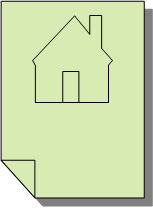
\includegraphics[width=0.25\textwidth]{figures/Homepage-icon.png}
  \end{center}
  \caption{Homepage icon}
  \label{fig:homepageicon}
\end{figure}

\begin{table}[!ht]
  \begin{center}
    \caption{Configurations tested}
    \label{tab:configstested}
    \begin{tabular}{l|c} % <-- Alignments: 1st column left, 2nd middle and 3rd right, with vertical lines in between
      \textbf{Configuration} & \textbf{Description} \\
      \hline
      1 & Simple test with one server\\
      2 & Simple test with one server\\
    \end{tabular}
  \end{center}
\end{table}
\todo[inline, backgroundcolor=kth-lightblue]{Testade konfigurationer}

\section{Implementation …/Modeling/Simulation/…}
\label{sec:implementationDetails}
\todo[inline, backgroundcolor=kth-lightblue]{Implementering … / modellering / simulering / …}


\subsection{Some examples of coding}

Listing~\ref{lst:helloWorldInC} shows an example of a simple program written
in C code.

\begin{lstlisting}[language={C}, caption={Hello world in C code}, label=lst:helloWorldInC]
int main() {
printf("hello, world");
return 0;
}
\end{lstlisting}


In contrast, Listing~\ref{lst:programmes} is an example of code in Python to
get a list of all of the programs at KTH.

\lstset{extendedchars=true}
\begin{lstlisting}[language={Python}, caption={Using a python program to
    access the KTH API to get all of the programs at KTH}, label=lst:programmes]
KOPPSbaseUrl = 'https://www.kth.se'

def v1_get_programmes():
    global Verbose_Flag
    #
    # Use the KOPPS API to get the data
    # note that this returns XML
    url = "{0}/api/kopps/v1/programme".format(KOPPSbaseUrl)
    if Verbose_Flag:
        print("url: " + url)
    #
    r = requests.get(url)
    if Verbose_Flag:
        print("result of getting v1 programme: {}".format(r.text))
    #
    if r.status_code == requests.codes.ok:
        return r.text           # simply return the XML
    #
    return None
\end{lstlisting}


\cleardoublepage
\chapter{Results and Analysis}
\label{ch:resultsAndAnalysis}
\todo[inline, backgroundcolor=kth-lightblue]{svensk: Resultat och Analys}

\todo[inline]{
Sometimes this is split into two chapters.\\
  
Keep in mind: How you are going to evaluate what you have done? What are your metrics?\\
Analysis of your data and proposed solution\\
Does this meet the goals which you had when you started?
}

In this chapter, we present the results and discuss them.

\todo[inline, backgroundcolor=kth-lightblue]{I detta kapitel presenterar vi resultaten och diskutera dem.\\
Ibland delas detta upp i två kapitel.\\
Hur du ska utvärdera vad du har gjort? Vad är din statistik?\\
Analys av data och föreslagen lösning\\
Innebär detta att uppfyllelse av de mål som du hade när du började?
}

\section{Major results}
\todo[inline, backgroundcolor=kth-lightblue]{Huvudsakliga resultat}

Some statistics of the delay measurements are shown in Table~\ref{tab:delayMeasurements}.
The delay has been computed from the time the GET request is received until the response is sent.

\todo[inline, backgroundcolor=kth-lightblue]{Lite statistik av fördröjningsmätningarna visas i Tabell~\ref{tab:delayMeasurements}. Förseningen har beräknats från den tidpunkt då begäran GET tas emot fram till svaret skickas.}

\begin{table}[!ht]
  \begin{center}
    \caption{Delay measurement statistics}
    \label{tab:delayMeasurements}
    \begin{tabular}{l|S[table-format=4.2]|S[table-format=3.2]} % <-- Alignments: 1st column left, 2nd middle and 3rd right, with vertical lines in between
      \textbf{Configuration} & \textbf{Average delay (ns)} & \textbf{Median delay (ns)}\\
      \hline
      1 & 467.35 & 450.10\\
      2 & 1687.5 & 901.23\\
    \end{tabular}
  \end{center}
\end{table}
\todo[inline, backgroundcolor=kth-lightblue]{Fördröj mätstatistik}
\todo[inline, backgroundcolor=kth-lightblue]{Konfiguration | Genomsnittlig fördröjning (ns) | Median fördröjning (ns)}

Figure \ref{fig:processing_vs_payload_length} shows and example of the
performance as measured in the experiments.

\begin{figure}[!ht]
% GNUPLOT: LaTeX picture
\setlength{\unitlength}{0.240900pt}
\ifx\plotpoint\undefined\newsavebox{\plotpoint}\fi
\begin{picture}(1500,900)(0,0)
\sbox{\plotpoint}{\rule[-0.200pt]{0.400pt}{0.400pt}}%
\put(171.0,131.0){\rule[-0.200pt]{4.818pt}{0.400pt}}
\put(151,131){\makebox(0,0)[r]{ 1.5}}
\put(1419.0,131.0){\rule[-0.200pt]{4.818pt}{0.400pt}}
\put(171.0,212.0){\rule[-0.200pt]{4.818pt}{0.400pt}}
\put(151,212){\makebox(0,0)[r]{ 2}}
\put(1419.0,212.0){\rule[-0.200pt]{4.818pt}{0.400pt}}
\put(171.0,292.0){\rule[-0.200pt]{4.818pt}{0.400pt}}
\put(151,292){\makebox(0,0)[r]{ 2.5}}
\put(1419.0,292.0){\rule[-0.200pt]{4.818pt}{0.400pt}}
\put(171.0,373.0){\rule[-0.200pt]{4.818pt}{0.400pt}}
\put(151,373){\makebox(0,0)[r]{ 3}}
\put(1419.0,373.0){\rule[-0.200pt]{4.818pt}{0.400pt}}
\put(171.0,454.0){\rule[-0.200pt]{4.818pt}{0.400pt}}
\put(151,454){\makebox(0,0)[r]{ 3.5}}
\put(1419.0,454.0){\rule[-0.200pt]{4.818pt}{0.400pt}}
\put(171.0,534.0){\rule[-0.200pt]{4.818pt}{0.400pt}}
\put(151,534){\makebox(0,0)[r]{ 4}}
\put(1419.0,534.0){\rule[-0.200pt]{4.818pt}{0.400pt}}
\put(171.0,615.0){\rule[-0.200pt]{4.818pt}{0.400pt}}
\put(151,615){\makebox(0,0)[r]{ 4.5}}
\put(1419.0,615.0){\rule[-0.200pt]{4.818pt}{0.400pt}}
\put(171.0,695.0){\rule[-0.200pt]{4.818pt}{0.400pt}}
\put(151,695){\makebox(0,0)[r]{ 5}}
\put(1419.0,695.0){\rule[-0.200pt]{4.818pt}{0.400pt}}
\put(171.0,776.0){\rule[-0.200pt]{4.818pt}{0.400pt}}
\put(151,776){\makebox(0,0)[r]{ 5.5}}
\put(1419.0,776.0){\rule[-0.200pt]{4.818pt}{0.400pt}}
\put(171.0,131.0){\rule[-0.200pt]{0.400pt}{4.818pt}}
\put(171,90){\makebox(0,0){ 0}}
\put(171.0,756.0){\rule[-0.200pt]{0.400pt}{4.818pt}}
\put(298.0,131.0){\rule[-0.200pt]{0.400pt}{4.818pt}}
\put(298,90){\makebox(0,0){ 10}}
\put(298.0,756.0){\rule[-0.200pt]{0.400pt}{4.818pt}}
\put(425.0,131.0){\rule[-0.200pt]{0.400pt}{4.818pt}}
\put(425,90){\makebox(0,0){ 20}}
\put(425.0,756.0){\rule[-0.200pt]{0.400pt}{4.818pt}}
\put(551.0,131.0){\rule[-0.200pt]{0.400pt}{4.818pt}}
\put(551,90){\makebox(0,0){ 30}}
\put(551.0,756.0){\rule[-0.200pt]{0.400pt}{4.818pt}}
\put(678.0,131.0){\rule[-0.200pt]{0.400pt}{4.818pt}}
\put(678,90){\makebox(0,0){ 40}}
\put(678.0,756.0){\rule[-0.200pt]{0.400pt}{4.818pt}}
\put(805.0,131.0){\rule[-0.200pt]{0.400pt}{4.818pt}}
\put(805,90){\makebox(0,0){ 50}}
\put(805.0,756.0){\rule[-0.200pt]{0.400pt}{4.818pt}}
\put(932.0,131.0){\rule[-0.200pt]{0.400pt}{4.818pt}}
\put(932,90){\makebox(0,0){ 60}}
\put(932.0,756.0){\rule[-0.200pt]{0.400pt}{4.818pt}}
\put(1059.0,131.0){\rule[-0.200pt]{0.400pt}{4.818pt}}
\put(1059,90){\makebox(0,0){ 70}}
\put(1059.0,756.0){\rule[-0.200pt]{0.400pt}{4.818pt}}
\put(1185.0,131.0){\rule[-0.200pt]{0.400pt}{4.818pt}}
\put(1185,90){\makebox(0,0){ 80}}
\put(1185.0,756.0){\rule[-0.200pt]{0.400pt}{4.818pt}}
\put(1312.0,131.0){\rule[-0.200pt]{0.400pt}{4.818pt}}
\put(1312,90){\makebox(0,0){ 90}}
\put(1312.0,756.0){\rule[-0.200pt]{0.400pt}{4.818pt}}
\put(1439.0,131.0){\rule[-0.200pt]{0.400pt}{4.818pt}}
\put(1439,90){\makebox(0,0){ 100}}
\put(1439.0,756.0){\rule[-0.200pt]{0.400pt}{4.818pt}}
\put(171.0,131.0){\rule[-0.200pt]{0.400pt}{155.380pt}}
\put(171.0,131.0){\rule[-0.200pt]{305.461pt}{0.400pt}}
\put(1439.0,131.0){\rule[-0.200pt]{0.400pt}{155.380pt}}
\put(171.0,776.0){\rule[-0.200pt]{305.461pt}{0.400pt}}
\put(30,453){\rotatebox{-270}{\makebox(0,0){Processing time (ms)}}}
\put(805,29){\makebox(0,0){Payload size (bytes)}}
\put(868.0,131.0){\rule[-0.200pt]{0.400pt}{84.074pt}}
\put(995.0,131.0){\rule[-0.200pt]{0.400pt}{98.287pt}}
\put(1173.0,131.0){\rule[-0.200pt]{0.400pt}{118.041pt}}
\put(1325.0,131.0){\rule[-0.200pt]{0.400pt}{134.904pt}}
\put(1350.0,131.0){\rule[-0.200pt]{0.400pt}{137.795pt}}
\put(1439.0,131.0){\rule[-0.200pt]{0.400pt}{155.380pt}}
\end{picture}
\caption[A GNUplot figure]{Processing time vs. payload length}\vspace{0.5cm}
\label{fig:processing_vs_payload_length}
\end{figure}
		

Given these measurements, we can calculate our processing bit rate as the inverse of the time it takes to process an additional byte divided by 8 bits per byte:

\[
	bitrate = \frac{1}{\frac{time_{byte}}{8}} = 20.03 \quad kb/s
\] 

\section{Reliability Analysis}
\todo[inline, backgroundcolor=kth-lightblue]{Analys av tillförlitlighet\\
Tillförlitlighet i metod och data}

\section{Validity Analysis}
\todo[inline, backgroundcolor=kth-lightblue]{Analys av validitet\\
Validitet i metod och data}

\cleardoublepage
\chapter{Discussion}
\label{ch:discussion}
\todo[inline, backgroundcolor=kth-lightblue]{Diskussion\\
Förbättringsförslag?}
\todo[inline]{This can be a separate chapter or a section
  in the previous chapter.}

\cleardoublepage
\chapter{Conclusions and Future work}
\label{ch:conclusionsAndFutureWork}
\todo[inline, backgroundcolor=kth-lightblue]{Slutsats och framtida arbete}

\todo[inline]{Add text to introduce the subsections of this chapter.}

\section{Conclusions}
\label{sec:conclusions}
\todo[inline, backgroundcolor=kth-lightblue]{Slutsatser}
\todo[inline]{Describe the conclusions (reflect on the whole introduction given in Chapter 1).}


  
\todo[inline]{Discuss the positive effects and the drawbacks.\\
Describe the evaluation of the results of the degree project.\\
Did you meet your goals?\\
What insights have you gained?\\
What suggestions can you give to others working in this area?\\
If you had it to do again, what would you have done differently?}

\todo[inline, backgroundcolor=kth-lightblue]{Uppfyllde du dina mål?\\
Vilka insikter har du fått?\\
Vilka förslag kan du ge till andra som arbetar inom detta område?
Om du skulle göra detta igen, vad skulle du ha gjort annorlunda?}

\section{Limitations}
\label{sec:limitations}
\todo[inline, backgroundcolor=kth-lightblue]{Begränsande faktorer\\
Vad gjorde du som begränsade dina ansträngningar? Vilka är begränsningarna i dina resultat?}
\todo[inline]{What did you find that limited your
  efforts? What are the limitations of your results?}


\section{Future work}
\label{sec:futureWork}
\todo[inline, backgroundcolor=kth-lightblue]{Vad du har kvar ogjort?\\
Vad är nästa självklara saker som ska göras?\\
Vad tips kan du ge till nästa person som kommer att följa upp på ditt arbete?
\todo[inline]{Describe valid future work that you or someone else could or should do.\\
Consider: What you have left undone? What are the next obvious things to be done? What hints can you give to the next person who is going to follow up on your work?
}

}


Due to the breadth of the problem, only some of the initial goals have been
met. In these section we will focus on some of the remaining issues that
should be addressed in future work. ...

\subsection{What has been left undone?}
\label{what-has-been-left-undone}

The prototype does not address the third requirment, i.e., a yearly
unavailability of less than 3 minutes, this remains an open problem. ...

\subsubsection{Cost analysis}

The current prototype works, but the performance from a cost perspective makes
this an impractical solution. Future work must reduce the cost of this
solution, to do so a cost analysis needs to first be done. ...

\subsubsection{Security}

A future research effort is needed to address the security holes that results
from using a self-signed certificate. Page filling text mass. Page filling
text mass. ...


\subsection{Next obvious things to be done}

In particular, the author of this thesis wishes to point out xxxxxx remains as
a problem to be solved. Solving this problem is the next thing that should be
done. ...

\section{Reflections}
\label{sec:reflections}
\todo[inline, backgroundcolor=kth-lightblue]{Reflektioner}
\todo[inline, backgroundcolor=kth-lightblue]{Vilka är de relevanta ekonomiska, sociala, miljömässiga och etiska aspekter av ditt arbete?}
\todo[inline]{What are the relevant economic, social,
  environmental, and ethical aspects of your work?
}



One of the most important results is the reduction in the amount of
energy required to process each packet while at the same time reducing the
time required to process each packet.

The thesis contributes to the \gls{UN}\enspace\glspl{SDG} numbers 1 and 9 by
xxxx. 